\chapter{Validated Results}
\label{cha:results}

To demonstrate our geo-based mediaplayer, we went out and did some recordings to test every functionality we’ve been working in the mediaplayer on during this project. We went to “Blåa havet” in front of Kårallen located at Linköping Universitet where some students were promoting an upcoming event with some activities. We found that this was a suitable point of interest to record from different angles for our testing case. As we only had two cameras available we made three sets of recordings consisting of two recordings each, with each set displaying the same scene from two different locations and angles at the same time. The desired outcome of this test was to be able to swap between the recordings to view the same object at one point in time from different angles.

\section{Position Algorithm}
\label{sec:positionalgorithm}

To demonstrate the accuracy of our relative placement of geographical points in our interface, we noted the GPS-coordinates and angles at the used recording locations. We then input the coordinates into Google Maps as seen in Figure \ref{fig:googlemaps}, which we will here use as a reference to prove the accuracy of our placement algorithm. We then input the same latitude, longitude and angle values into our interface and the result is shown in Figure \ref{fig:testfallgeomap}.


\begin{figure}[ht!]
\begin{center}
	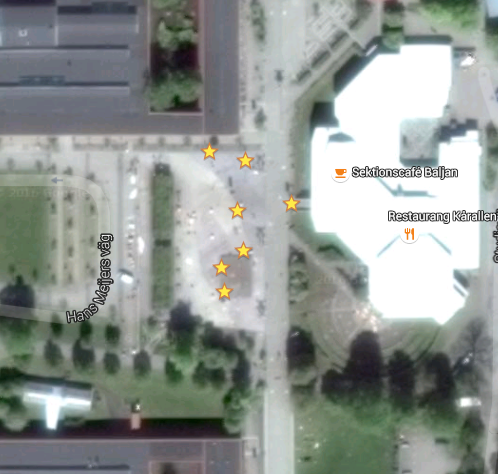
\includegraphics[scale=0.64]{Google_Maps.png}
	\caption{Google Maps view of the Streaming locations}
	\label{fig:googlemaps}
\end{center}
\end{figure}

\begin{figure}[ht!]
\begin{center}
	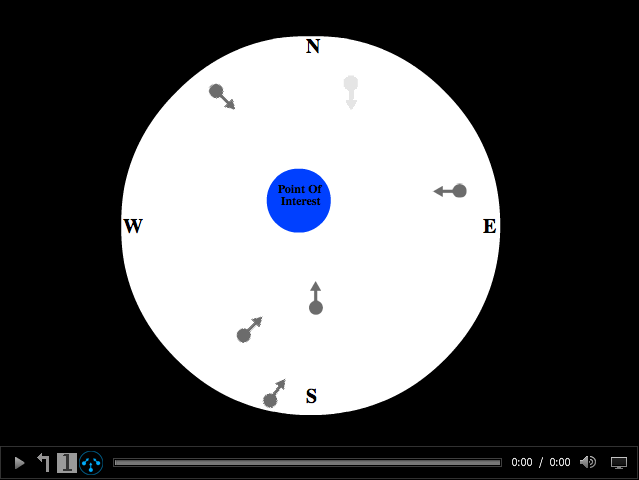
\includegraphics[scale=0.37]{TestfallGeomap.png}
	\caption{Geo-map view of the Streaming locations}
	\label{fig:testfallgeomap}
\end{center}
\end{figure}

The arrow-points in the geographic map is almost an exact match to those in the Google Maps screenshot, at least in terms in relativity. There is a slight difference between the two and the reason for this is that the points in our geographical map is scaled to make use the entire map, in such a way that the distance between them are increased while their relative locations between each other remain intact. This would prove the accuracy of our relative placement of the geographical points.

\section{Geo-based Streaming}
\label{sec:geobasedstreaming}

As we’ve mentioned before, our implementations is as shown in Figure \ref{fig:gpsinterface} where we have a button that opens the geographical map, a circle that represents a “map” and arrows pointing in a direction that represents streamers/videos. When a video is selected the arrow is highlighted and that video is then played. In our test case, we set up two cameras at a time and did recordings of 90 seconds each. In these videos we captured plenty of people doing plenty of stuff. There were people jumping the trampoline, using hoverboards, walking and biking around. When we input these 3 sets of two recordings each into our mediaplayer, we could swap between the two recordings and watch these same events unfold from different positions and angles. In Figure \ref{fig:testview1} and \ref{fig:testview2} two different recordings are selected and they show the same event where, for example, the guy inside the red circle in the pictures are hoverboarding in front of the red shirt guy the same time. This would prove the desired functionality of where the user can display the same event from different geographical positions and angles.

\begin{figure}[ht!]
\begin{center}
	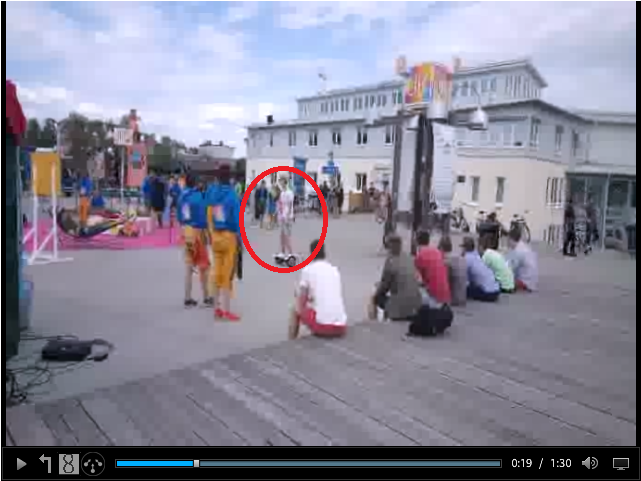
\includegraphics[scale=0.8]{Hoverboard_1.png}
	\caption{Test view 1}
	\label{fig:testview1}
\end{center}
\end{figure}

\begin{figure}[ht!]
\begin{center}
	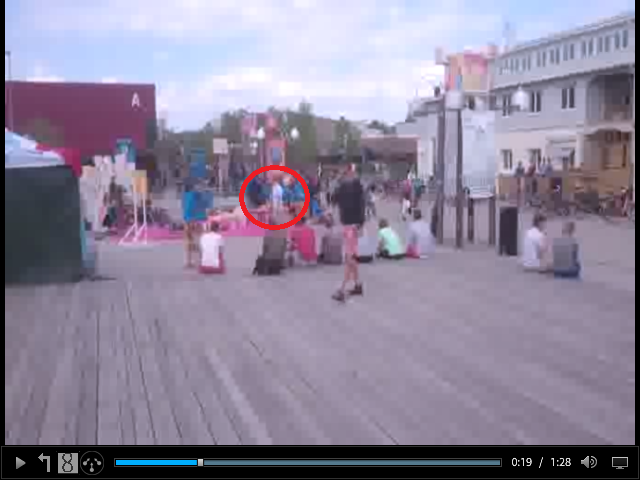
\includegraphics[scale=0.8]{Hoverboard_2.png}
	\caption{Test view 2}
	\label{fig:testview2}
\end{center}
\end{figure}